\section{Related work}\label{s:related}

\begin{figure}[t]
\centering
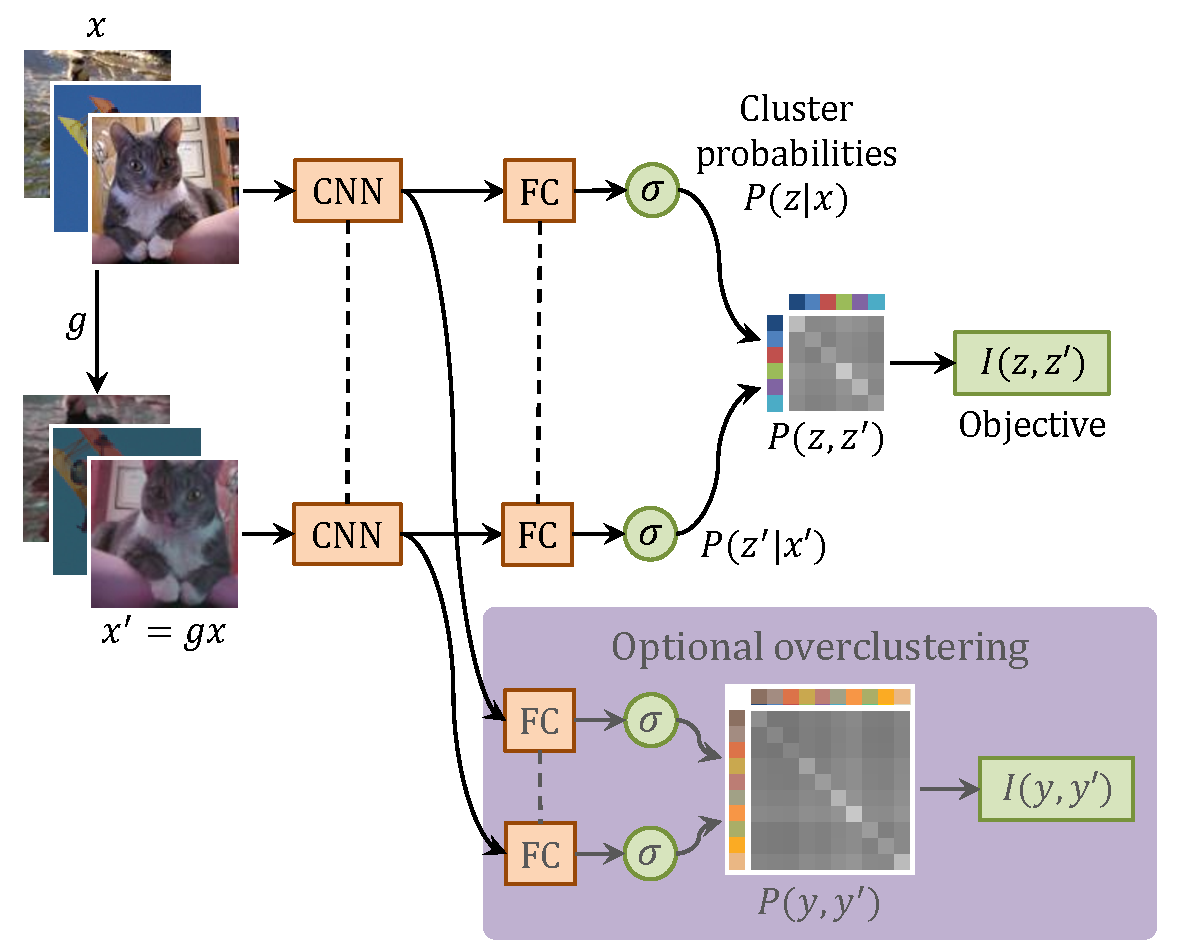
\includegraphics[width=0.95\columnwidth]{paper_imgs/overview1.pdf}
\caption{\label{f:overview}\methodnameshort for image clustering. Dashed line denotes shared parameters, $g$ is a random transformation, and $I$ denotes mutual information~(\cref{e:loss_expanded}).}
\end{figure}


\begin{figure*}
%\captionsetup{justification=centering}
\setlength\tabcolsep{2.2pt} % default value: 6pt

\begin{tabular}{c c c c c c}
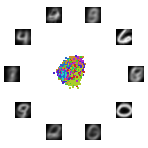
\includegraphics[height=0.16\textwidth]{experiments2_files/mnist_progression/726_run_1_colour_0_pointcloud_0.png} & 
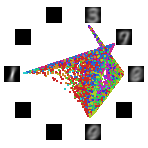
\includegraphics[height=0.16\textwidth]{experiments2_files/mnist_progression/726_run_1_colour_0_pointcloud_3.png} & 
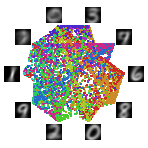
\includegraphics[height=0.16\textwidth]{experiments2_files/mnist_progression/726_run_1_colour_0_pointcloud_10.png} & 
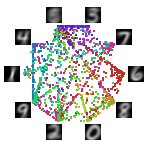
\includegraphics[height=0.16\textwidth]{experiments2_files/mnist_progression/726_run_1_colour_0_pointcloud_30.png} & 
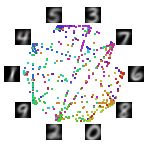
\includegraphics[height=0.16\textwidth]{experiments2_files/mnist_progression/726_run_1_colour_0_pointcloud_101.png} & 
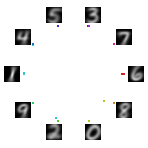
\includegraphics[height=0.16\textwidth]{experiments2_files/mnist_progression/726_run_1_colour_0_pointcloud_1000.png} 
\end{tabular}

\caption{\label{f:mnist_dots} Training with \methodnameshort on unlabelled MNIST in successive epochs from random initialisation (left). The network directly outputs cluster assignment probabilities for input images, and each is rendered as a coordinate by convex combination of 10 cluster vertices. There is no cherry-picking as the entire dataset is shown in every snapshot. Ground truth labelling (unseen by model) is given by colour. At each cluster the average image of its assignees is shown. With neither labels nor heuristics, the clusters discovered by \methodnameshort correspond perfectly to unique digits, with one-hot certain prediction (right).}
\end{figure*}


\paragraph{Co-clustering and mutual information.}

The use of information as a criterion to learn representations is not new. One of the earliest works to do so is by Becker and Hinton~\cite{becker1992self}.
More generally, learning from paired data has been explored in co-clustering~\cite{hartigan1972direct, dhillon2003information} and in other works~\cite{wang2010information} that build on the information bottleneck principle~\cite{friedman2001multivariate}.

Several recent papers have used information as a tool to train deep networks in particular.
IMSAT~\cite{hu2017learning} maximises mutual information between data and its representation and DeepINFOMAX~\cite{hjelm2018learning} maximizes information between spatially-preserved features and compact features.
However, IMSAT and DeepINFOMAX combine information with other criteria, whereas in our method information is the only criterion used.
Furthermore, both IMSAT and DeepINFOMAX compute mutual information over continuous random variables, which requires complex estimators~\cite{belghazi2018mine}, whereas \methodnameshort does so for discrete variables with simple and exact computations.
Finally, DeepINFOMAX considers the information $I(\bx, f(\bx))$ between the features $\bx$ and a deterministic function $f(\bx)$ of it, which is in principle the same as the entropy $H(\bx)$; in contrast, in \methodnameshort information does not trivially reduce to  entropy.

\paragraph{Semantic clustering versus intermediate representation learning.}
In semantic clustering, the learned function directly outputs discrete assignments for high level (i.e. semantic) clusters. Intermediate representation learners, on the other hand, produce continuous, distributed, high-dimensional representations that must be post-processed, for example by k-means, to obtain the discrete low-cardinality assignments required for unsupervised semantic clustering. The latter includes objectives such as generative autoencoder image reconstruction~\cite{vincent2010stacked},  triplets~\cite{schultz2004learning} and spatial-temporal order or context prediction~\cite{lee2017unsupervised,cruz2017deeppermnet,doersch2015unsupervised}, for example predicting patch proximity~\cite{isola2015learning}, solving jigsaw puzzles~\cite{noroozi2016unsupervised} and inpainting~\cite{pathak2016context}. Note it also includes a number of clustering methods (DeepCluster~\cite{caron2018deep}, exemplars~\cite{dosovitskiy2015discriminative}) where the clustering is only auxiliary; a clustering-style objective is used but does not produce groups with semantic correspondence. For example, DeepCluster~\cite{caron2018deep} is a state-of-the-art method for learning highly-transferable intermediate features using overclustering as a proxy task, but does not automatically find semantically meaningful clusters. As these methods use auxiliary objectives divorced from the semantic clustering objective, it is unsurprising that they perform worse than \methodnameshort~(\cref{s:experiments}), which directly optimises for it, training the network end-to-end with the final clusterer implicitly wrapped inside.




\paragraph{Optimising image-to-image distance.}

Many approaches to deep clustering, whether semantic or auxiliary, utilise a distance function between input images that approximates a given grouping criterion.
Agglomerative clustering~\cite{bautista2016cliquecnn} and partially ordered sets~\cite{bautista2017deep} of HOG features~\cite{dalal2005histograms} have been used to group images, and exemplars~\cite{dosovitskiy2015discriminative} define a group as a set of random transformations applied to a single image. Note the latter does not scale easily, in particular to image segmentation where a single $200\times 200$ image would call for 40k classes. DAC~\cite{chang2017deep}, JULE~\cite{yang2016joint}, DeepCluster~\cite{caron2018deep}, ADC~\cite{haeusser2018associative} and DEC~\cite{xie2016unsupervised} rely on the inherent visual consistency and disentangling properties~\cite{greff2015binding} of CNNs to produce cluster assignments, which are processed and reinforced in each iteration. 
The latter three are based on k-means style mechanisms to refine feature centroids, which is prone to degenerate solutions~\cite{caron2018deep} and thus needs explicit prevention mechanisms such as pre-training, cluster-reassignment or feature cleaning via PCA and whitening~\cite{xie2016unsupervised, caron2018deep}.

\begin{comment}
DAC is the only unsupervised clustering algorithm out of these that eschews k-means and agglomerative clustering for a different but similar clustering scheme, based on feature inner-products rather than distances.
DAC forms clusters gradually, in a self-paced manner, thus alleviating but not eliminating the risk of incurring degenerate solutions.
Furthermore, the nature of the optimisation, which reinforces bootstrapped class labels, creates a strong dependency on initialisation.

For unsupervised feature learning in general, i.e.\ where the training objective is not clustering, a large number of works explore using proxy learning tasks. 
There are two major directions:  generative tasks such as autoencoder image reconstruction~\cite{vincent2010stacked}, and spatial-temporal order or context prediction~\cite{lee2017unsupervised,cruz2017deeppermnet,doersch2015unsupervised}. The latter includes predicting patch proximity~\cite{isola2015learning}, solving jigsaw puzzles~\cite{noroozi2016unsupervised} and inpainting~\cite{pathak2016context}. 
In many cases they benefit from principled formulations that protect against degeneracy.
However, unlike the aforementioned clustering methods, the features learned by these methods need to be post-processed, for example using k-means, to cluster the data. 

\end{comment}

\paragraph{Invariance as a training objective.}

Optimising for function outputs to be persistent through spatio-temporal or non-material distortion is an idea shared by \methodnameshort with several works, including exemplars~\cite{dosovitskiy2015discriminative}, IMSAT~\cite{hu2017learning}, proximity prediction~\cite{isola2015learning}, the denoising objective of Tagger~\cite{greff2016tagger}, temporal slowness constraints~\cite{zou2012deep}, and optimising for features to be invariant to local image transformations~\cite{sohn2012learning,hui2013direct}.
More broadly, the problem of modelling data transformation has received significant attention in deep learning, one example being the transforming autoencoder~\cite{hinton2011transforming}.


% \section{Related work}\label{s:related}

% \paragraph{Co-clustering and mutual information.}

% The idea of learning a data representation by seeking the common parts of related observations is not new. 
% An early work is Becker and Hinton~\cite{becker1992self}, which maximises agreement between representations of 2D images to learn depth, using an objective corresponding to maximising mutual information between the input and the average of the data representations. 
% Co-learning has also been explored in the context of clustering by co-clustering methods, dating back to the pioneering work of Hartigan~\cite{hartigan72direct}. 
% Many information-theoretic variant of such approaches have been proposed, as discussed by~\cite{wang10information}, which are generally related to the information bottleneck principle~(\cite{friedman2001multivariate}). 

% A few works have employed mutual information in the context of unsupervised deep learning. IMSAT~\cite{hu2017learning} maximises mutual information between input data and their predicted discrete representations whilst encouraging the representations of augmented data points to be close to those of the original data points. 
% DeepINFOMAX~\cite{hjelm2018learning} maximises mutual information between spatially preserved features and compact features. There are some major differences with \methodnameshort. 
% Firstly, mutual information is used as an aid in these methods, as it increases the statistical predictivity between two random variables. 
% This contrasts with our method, where mutual information constitutes the loss applied directly to cluster assignments, meaning it is used as a clustering objective. 
% Secondly, both IMSAT and DeepINFOMAX compute mutual information over continuous random variables, which calls for an integral and is not computationally tractable, so estimators~\cite{belghazi2018mine} are used. 
% Since \methodnameshort maximises mutual information between cluster assignments and the number of clusters is discrete, computation is exact and straightforward. 
% Finally, DeepINFOMAX employs mutual information between function inputs and outputs, i.e. $I(x, f(x))$, but the conditional entropy component of mutual information $H(f(x) | x)$ is 0 when $f$ is deterministic, making the maximisation less meaningful. 
% In contrast \methodnameshort maximises mutual information between cluster assignments of separate images, i.e. $I(z, z')$ where $z$ and $z'$ are not functions of one other, making $H(z | z')$ a non-zero quantity that contributes to the optimisation as it can be minimised.

% \paragraph{Optimising image-to-image distance for clustering.}
% Many works for on unsupervised deep clustering involve establishing a scheme for estimating the semantic distance between input images, before training a function to learn this scheme. 
% CliqueCNN~\cite{bautista2016cliquecnn} trains a network to discriminate between cliques that are determined by applying agglomerative clustering on image features such as HOG~\cite{dalal2005histograms}. 
% In Exemplar CNNs~\cite{dosovitskiy2016discriminative}, each image and a its set of random transformations is considered a class, and a function is trained to discriminate between these surrogate classes. Like \methodnameshort, this method uses random transformations as a proxy for obtaining images with low semantic distance in the absence of label information. 
% Requiring one class per input image has a large memory footprint which makes Exemplar CNNs infeasible for segmentation (where patches are clustered instead of images, so a single 200x200 image would call for 40k classes). 

% \begin{figure}[t]
\centering
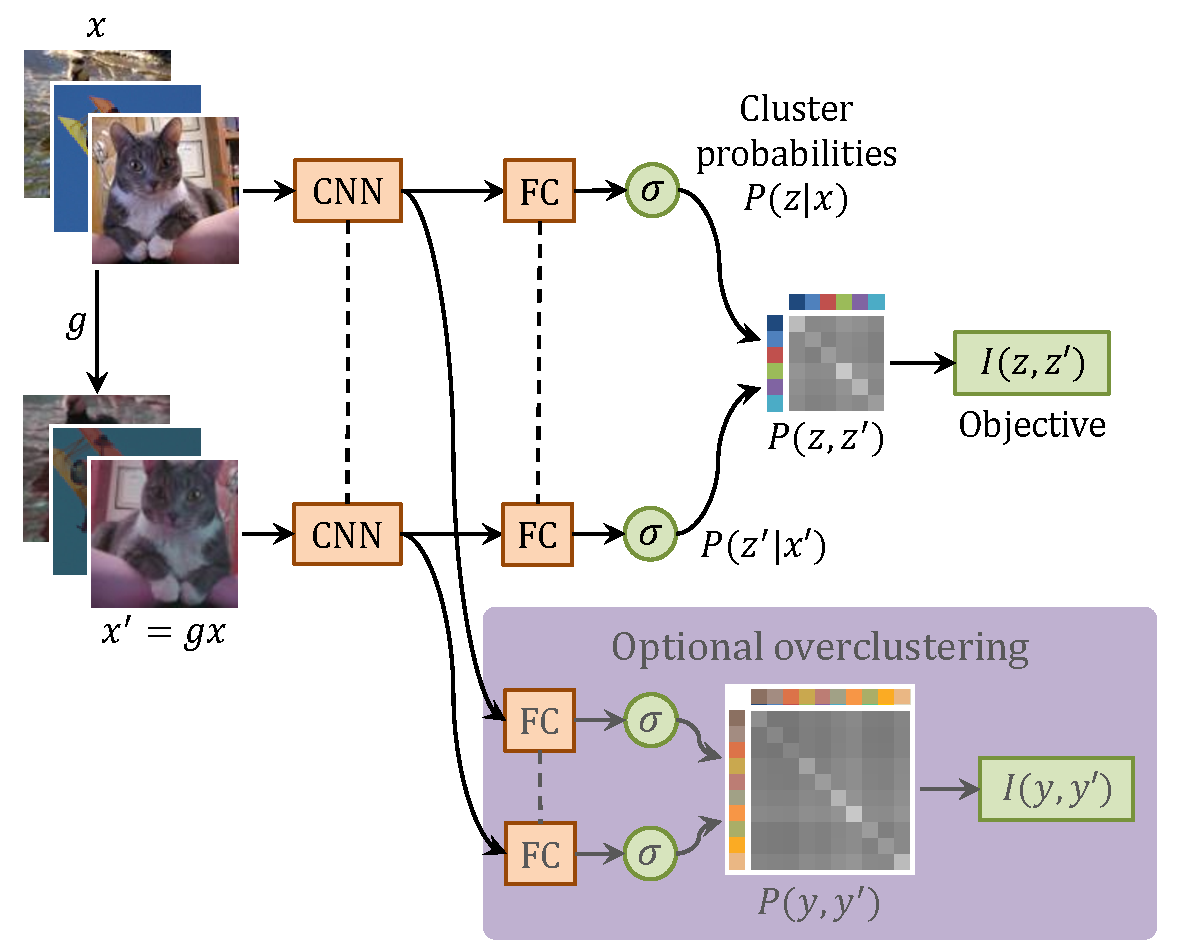
\includegraphics[width=0.95\columnwidth]{paper_imgs/overview1.pdf}
\caption{\label{f:overview}\methodnameshort for image clustering. Dashed line denotes shared parameters, $g$ is a random transformation, and $I$ denotes mutual information~(\cref{e:loss_expanded}).}
\end{figure}


% DAC~\cite{chang2017deep}, JULE~\cite{yang2016joint}, DeepCluster~\cite{caron2018deep}, Associative Deep Clustering~\cite{haeusser18associative} and DEC~\cite{xie2016unsupervised} all rely on the inherent visual consistency and disentangling properties~\cite{greff2015binding} of CNNs to produce meaningful cluster assignments, which are processed and reinforced in each iteration. 
% The latter three are based on using k-means to refine deep feature vectors, a mechanism which is prone to degenerate solutions~\cite{caron2018deep} and thus needs explicit prevention mechanisms such as pre-training, cluster-reassignment or feature cleaning via PCA and whitening ~\cite{xie2016unsupervised, caron2018deep}. 

% DAC is the only unsupervised clustering algorithm out of these that eschews k-means whilst training a network to directly produce cluster assignments, as \methodnameshort does. 
% A network is trained to produce cluster assignment probability distributions for each sample that are used as high level feature descriptors, and the dot product of different descriptors is treated as a proxy for inter-sample semantic distance (instead of Euclidian distance, which is used in the k-means based clusterers). 
% Training proceeds by maximising the dot product of close sample pairs, thus encouraging them to be assigned to the same cluster, whilst minimising the dot product for far pairs. 
% The nature of the optimisation means there is a strong dependency on initialisation and lack of protection against degenerate solutions such as clusters disappearing. 

% \paragraph{Proxy tasks for unsupervised feature learning.}
% For unsupervised feature learning in general, i.e. where the training objective is not clustering, a large number of works explore using proxy learning tasks. 
% There are two major camps:  generative tasks such as autoencoder image reconstruction~\cite{vincent2010stacked}, and spatial-temporal order or context prediction~\cite{lee2017unsupervised,cruz2017deeppermnet,doersch2015unsupervised}. The latter includes predicting patch proximity~\cite{isola2015learning}, solving jigsaw puzzles~(\cite{noroozi2016unsupervised}) and inpainting~(\cite{pathak2016context}). 
% In many cases they benefit from principled formulations that protect against degeneracy.
% However, unlike the aforementioned clustering methods, learned representations from these tasks constitute fine-grained continuous features rather than coarse cluster assignments, and thus must be post-processed, either by unsupervised clustering such as k-means or with label information via SVMs or fine-tuning, in order to produce semantic clusters.

% \paragraph{Invariance as a training objective.}
% Training for function outputs to be persistent through spatio-temporal distortion, noise distortion, or random transforms is an idea shared by \methodnameshort and several mentioned works, including Exemplar CNNs~\cite{dosovitskiy2016discriminative}, IMSAT~\cite{hu2017learning} and proximity prediction~\cite{isola2015learning}.
% It is also seen in Tagger~\cite{greff2016tagger}, which trains a function to denoise its input using several clusters to distribute the representation,~\cite{zou2012deep} which enforces a temporal slowness constraint on learned features, and~\cite{sohn2012learning,hui2013direct} which train for features invariant to local image transformations.


